\section{Glass and Silicon}
\label{sec:GlassAndSilicon}
In this section the absorption of glass and other media are discussed. Before starting the discussion, we have to 
recognize that glass is a brought term in this context for an amorphous solid without crystalline structure.
Its components and therefore its physical properties can widely vary.

Having said this, we explain the typical behaviour of standard glass using soda-lime glass as an example. As shown 
in Figure \ref{fig:SodaLimeGlass} transparent glass does not absorb in the visible range between \SI{1.3}{eV} - \SI{4}{eV}.

\begin{figure}[ht]
    \centering
    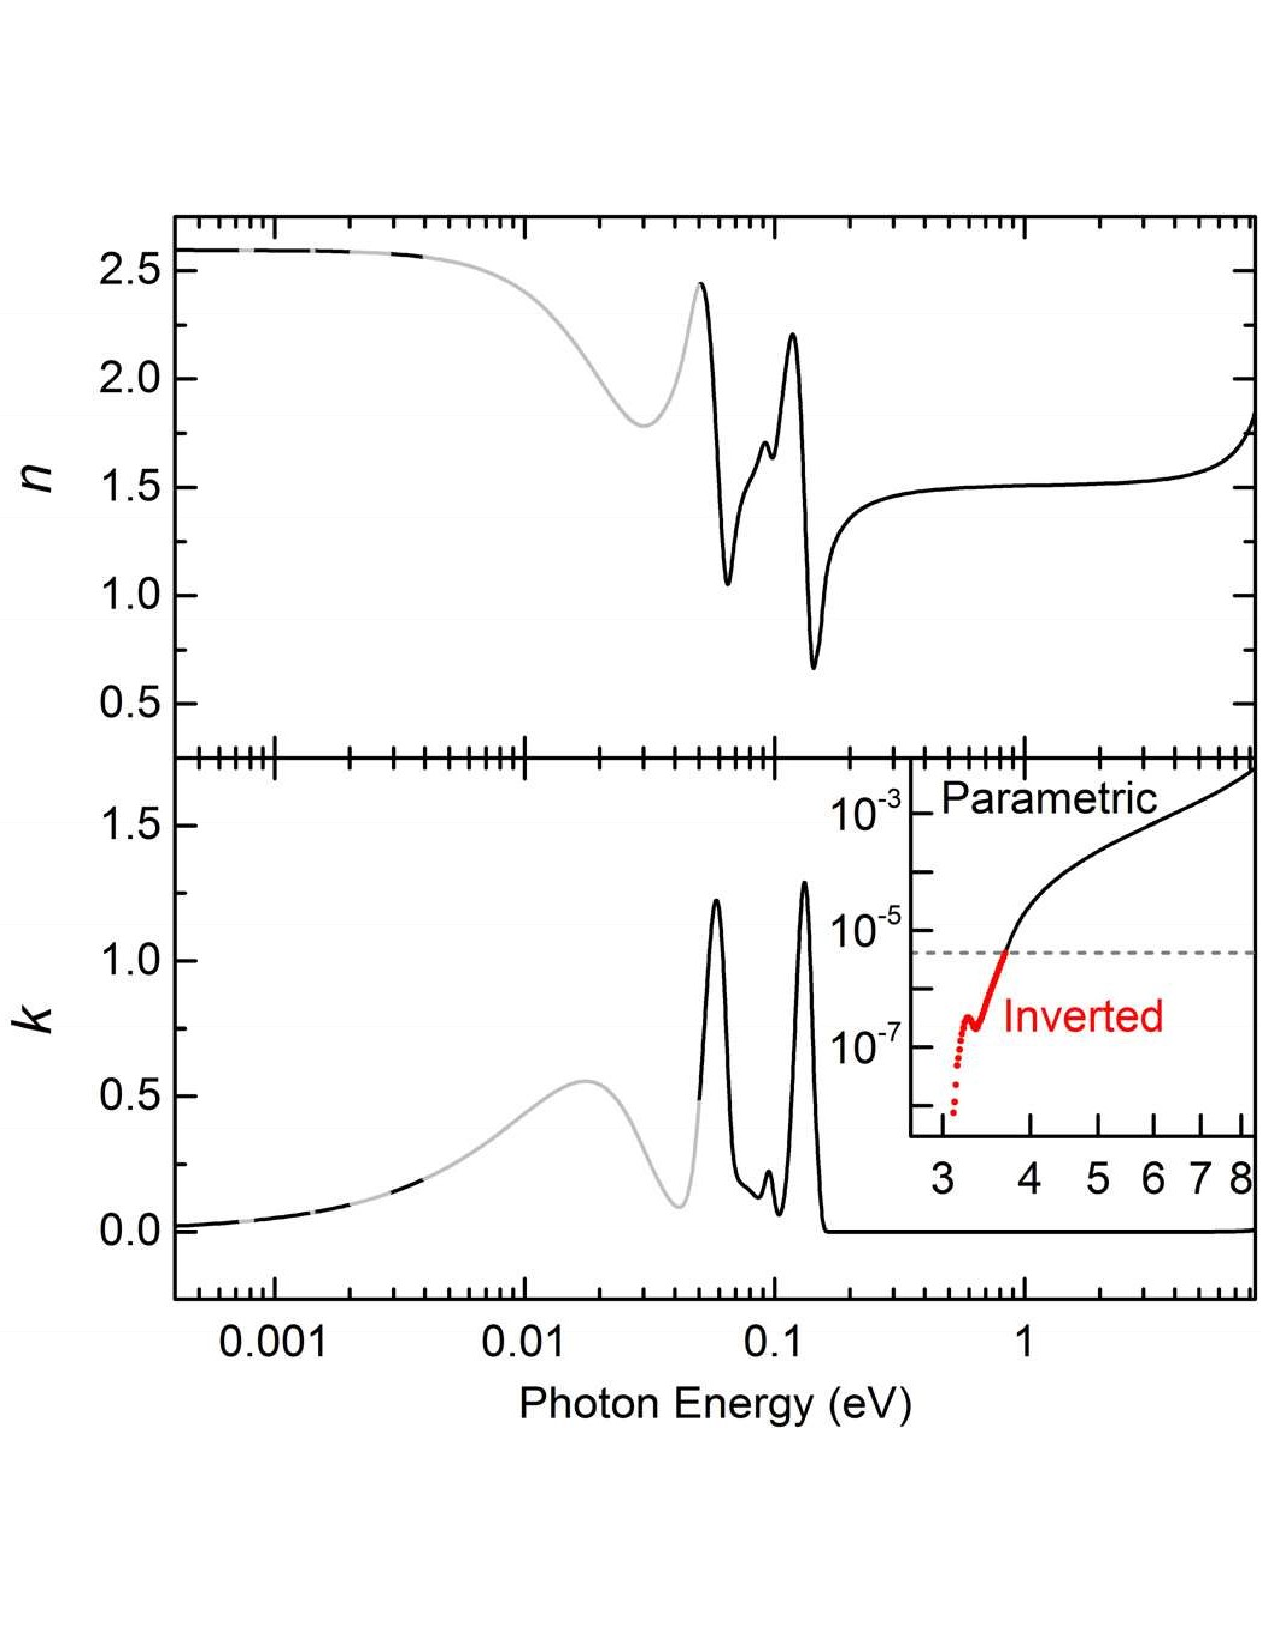
\includegraphics[width = 10cm]{Bilder/Grundlagen/SodalimePic.pdf}
    \caption{Spectra in N = n + ik describing the bulk soda lime glass layer over the full measured spectral range. The
    gray lines correspond to spectral regions where there are gaps in the measured spectra. The inset shows k generated
    by both parametric modeling and by numerical inversion over ranges of k where each is most sensitive. From \cite[]{Junda.2018}.}
    \label{fig:SodaLimeGlass}
\end{figure}

As seen in Figure \ref{fig:SodaLimeGlass} and described in section \ref{sec:dispersion} there is a close link through the Kramers-Kronig relations
between the optical extinction coefficient $\kappa$ and the refractive index. It can be seen 
that soda-lime glass -- as many glasses -- exhibits absorption in the ultraviolet (UV) range, since the refractive index 
shows the characteristic increase.  

%TODO #1
The difference in absorption in the spectral range observed later stresses the importance of a reference measurement.